\documentclass{beamer}
\usepackage{ctex, hyperref}
\usepackage[T1]{fontenc}

% other packages
\usepackage{latexsym,amsmath,xcolor,multicol,booktabs,calligra}
\usepackage{graphicx,pstricks,listings,stackengine,subfigure}

\author{袁雨辰\ 林华康\ 王贤义\ 陈鑫安}
\title{基于多无人机协同的草原修复方法研究}
\subtitle{国创项目答辩汇报}
\institute{兰州大学信息科学与工程学院}
\date{2023 年 9 月 28 日

}
\logo{

\includegraphics[scale=0.5]{pic/logo.png}
}
\usepackage{NJUPT}

\def\cmd#1{\texttt{\color{red}\footnotesize $\backslash$#1}}
\def\env#1{\texttt{\color{blue}\footnotesize #1}}
\definecolor{deepblue}{rgb}{0,0,0.5}
\definecolor{deepred}{rgb}{0.6,0,0}
\definecolor{deepgreen}{rgb}{0,0.5,0}
\definecolor{halfgray}{gray}{0.55}

\lstset{
    basicstyle=\ttfamily\small,
    keywordstyle=\bfseries\color{deepblue},
    emphstyle=\ttfamily\color{deepred},    % Custom highlighting style
    stringstyle=\color{deepgreen},
    numbers=left,
    numberstyle=\small\color{halfgray},
    rulesepcolor=\color{red!20!green!20!blue!20},
    frame=shadowbox,
}


\begin{document}

\kaishu
\begin{frame}
    \titlepage
    %\begin{figure}[htpb]
    % \begin{center}
    %  
\includegraphics[width=0.2\linewidth]{pic/logo.eps}
    %\end{center}
    %\end{figure}
\end{frame}
\begin{frame}
    \tableofcontents[sectionstyle=show,subsectionstyle=show/shaded/hide,subsubsectionstyle=show/shaded/hide]
\end{frame}


\section{项目背景}

\begin{frame}{项目背景}
    \begin{itemize}
        \item 草原是地球上最重要的陆地生态系统之一,被誉为“地球的皮肤”。草原既是农牧业发展的基础,也是生态安全的主要屏障,它在维护生态和保障民生等方面都发挥着至关重要的作用。对于生态而言,草原具有防风固沙、涵养水源、固碳释氧、调节气候、美化环境及维护生物多样性等重要功能。\cite{8249536}
        \item[]
              \begin{figure}[htbp]
                  \begin{minipage}{0.49\linewidth}
                      \centering
                      
\includegraphics[scale=0.2]{pic/1.png}
                      \caption{草原修复前}
                  \end{minipage}
                  \begin{minipage}{0.49\linewidth}
                      \centering
                      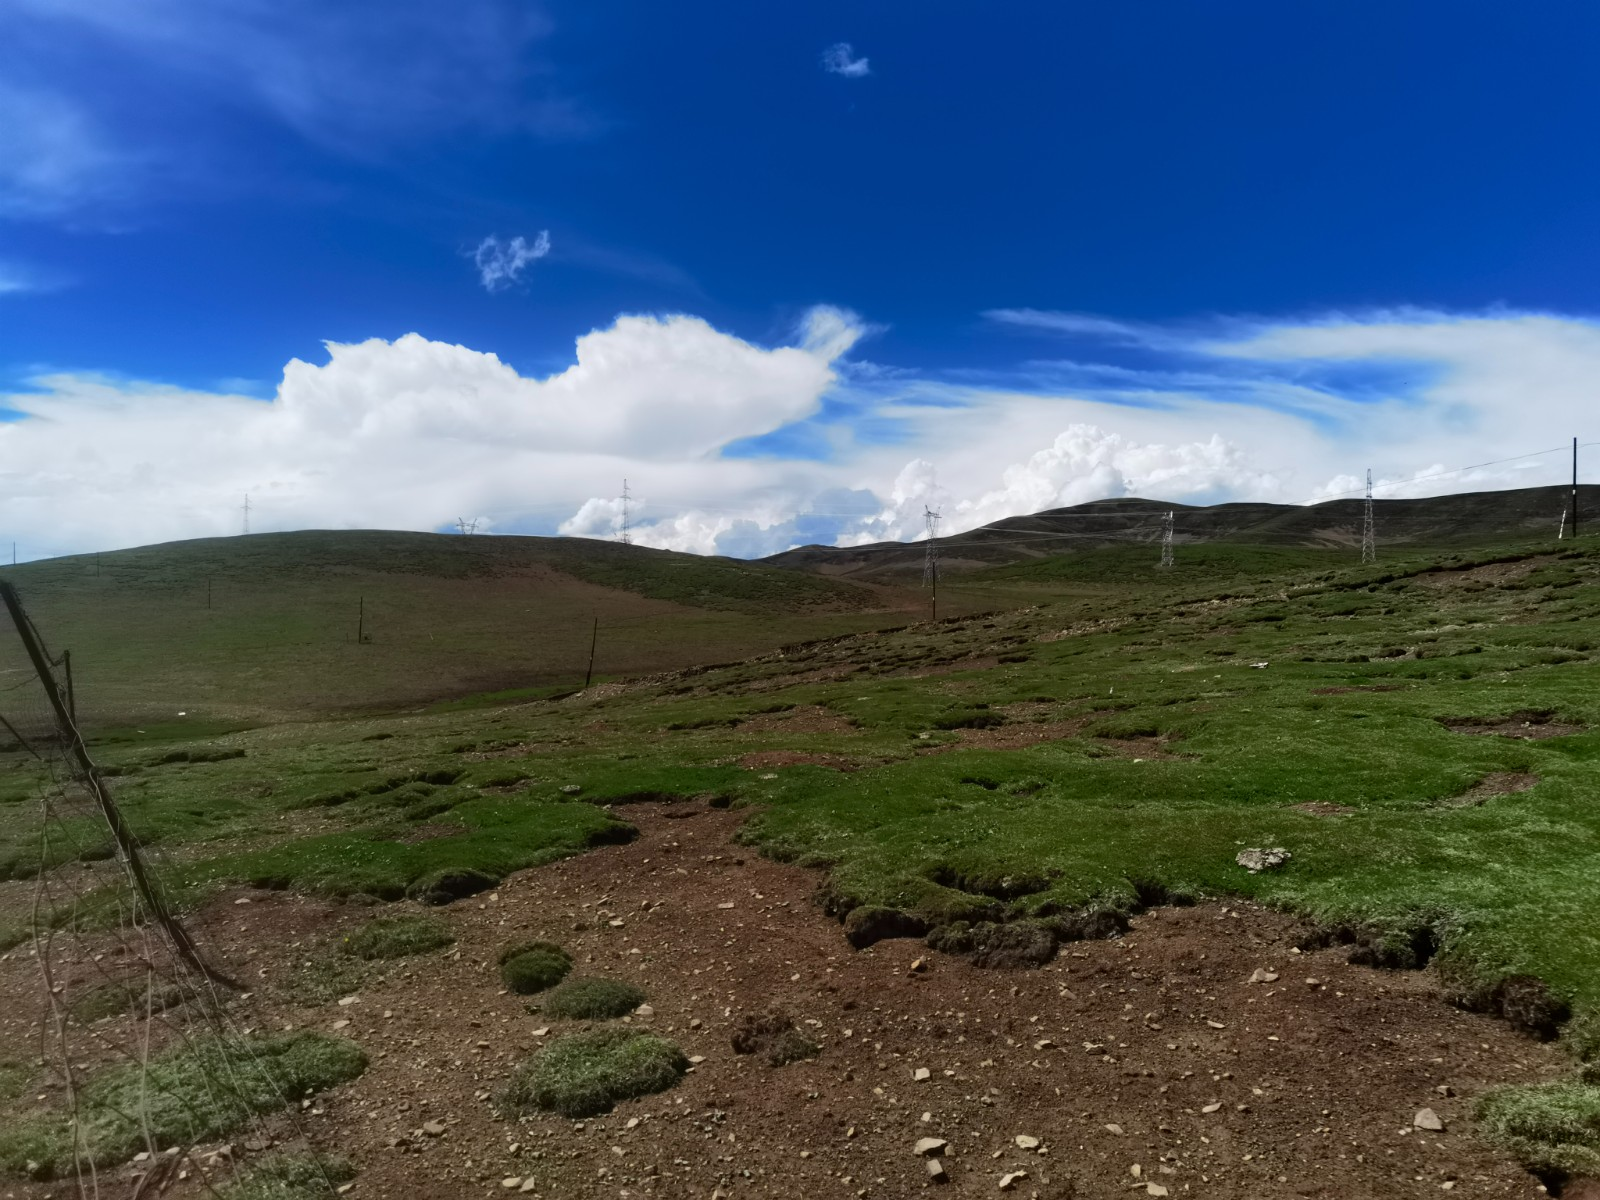
\includegraphics[scale=0.08]{pic/2.png}
                      \caption{草原修复后}
                  \end{minipage}
              \end{figure}
    \end{itemize}
\end{frame}

\begin{frame}{项目背景}
    \quad \quad 多UAV协同的草原修复方法是从草原修复的实际需求出发,结合草原生态环境特点和UAV发展的前沿技术提炼而成的。由于目前国内外针对多UAV协同的草原修复技术的研究工作尚不多见,本项目重点围绕草原信息化设备不完善、草原监测数据收集难度大等问题,尝试采用无人机作为移动数据收集设备,通过实时调度来实现监测数据收集。该项目为草原监测数据收集提供了切实可行的解决方案,有助于提升草原的智慧化水平,助力打造人、畜和自然和谐发展的生态系统。\cite{8470897}\cite{9018112}

    \begin{figure}[htbp]
        \centering
        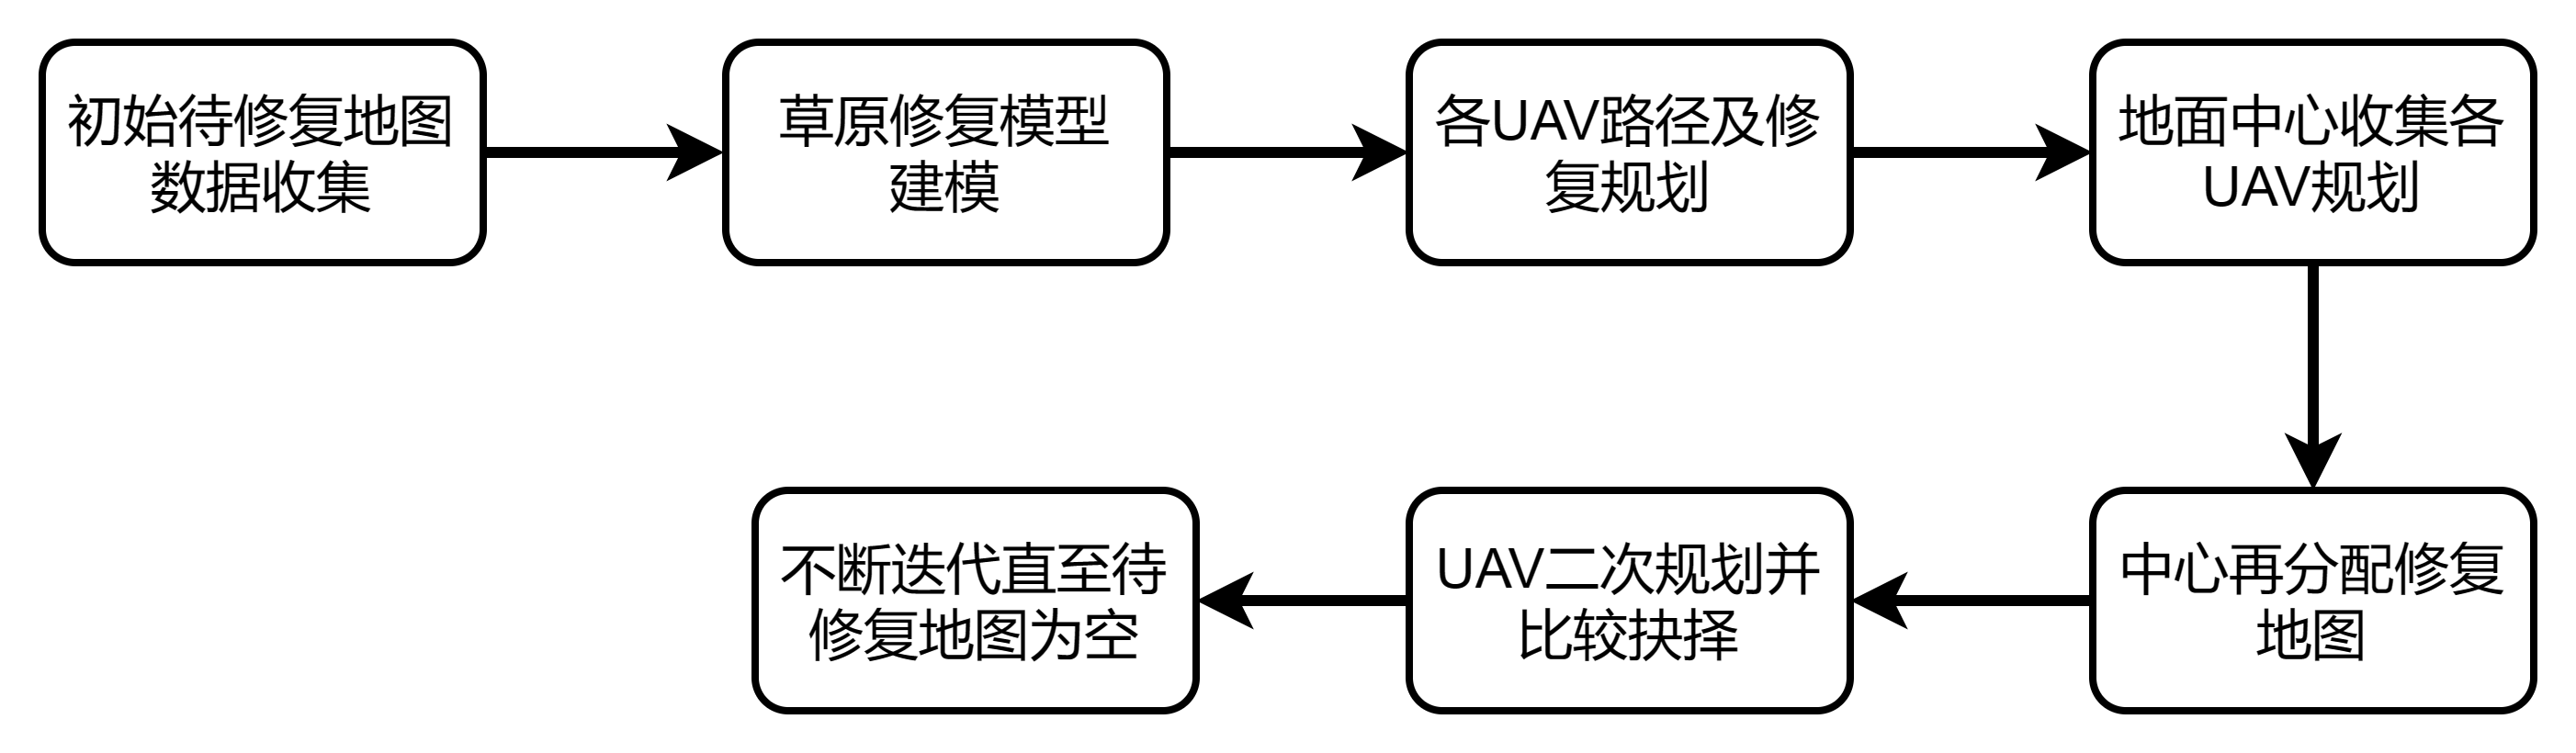
\includegraphics[scale=0.1]{pic/0.png}
    \end{figure}
\end{frame}

\begin{frame}{项目创新}
    \begin{itemize}
        \item 求解方法:本项目借鉴强化学习指针网络求解PCTSP问题的思路,通过对网络结构的创新设计求出问题的较优解。
        \item 模型创新:本项目利用了无人机作为移动数据收集设备,设计了基于无人机的监测数据收集模型,实现了草原监测数据的实时调度和收集,避免了传统人工收集方式中可能存在的误差和盲区。
        \item 算法创新:该项目设计了一种新的路径规划算法,能够根据监测设备的地理位置信息、已经过路径,快速决策出一条可行的路径,进一步提高了算法的效率和准确性。
    \end{itemize}
\end{frame}

\section{项目内容}

\begin{frame}{项目内容}
    \quad \quad 本项目中,多个 UAV 携带种子、信号收发装置、充满电的电池和草原待修复区域的信息(包括面积和退化等级)等从基站出发,依次飞入事先规划的待修复区域 访问每个待修复目标并进行修复作业,然后在保证有一定剩余能量时返回基站接受充电等服务,并为再次修复做准备,如图所示。
    \begin{figure}[htbp]
        \centering
        
\includegraphics[scale=0.3]{pic/3.png}
        \caption{多UAV协同的草原修复示意图}
    \end{figure}
\end{frame}

\begin{frame}{数学模型}
    通过文献调研与约束设置,本项目建立数学模型如下:
    \begin{subequations}
        \begin{align}
            \min  \sum_{j, k} r_{k} n_{k} \frac{V_{j}}{\theta_{j}}\left(x_{k j} -\theta_{j}\right)^{2} +\sum_{j} p_{j} u_{j} - \lambda \sum_{j, k} r_{k} n_{k} x_{k j} c_{k j}  \ \ \tag{\ref{eq:ctr_shale}}
        \end{align}
        \begin{alignat}{2}
            \text{s.t.} & \sum_{k \in \Gamma(j)} r_{k} n_{k} x_{k j}+u_{j}  \geq d_{j}, \forall j & \text{ (demand constraints)}        \\
                        & \sum_{j \in \Gamma(k)} x_{k j} \leq 1, \ \forall k                      & \text{(supply constraints)}         \\
                        & r_{k} x_{k j} \leq f_{j}, \ \forall k,j                                 & \text{ (frequency constraints)}     \\
                        & n_{k} x_{k j}  \leq 1, \ \forall k, j                                   & \text{ (slot constraints)}          \\
                        & x_{k j}, u_j\ge 0, \  \forall k, j                                      & \text{ (non-negativity constraint)}
        \end{alignat}
    \end{subequations}
\end{frame}

\section{项目方案}

\begin{frame}{项目方案}
    本项目拟围绕退化草原修复问题,通过研究UAV赋能的草原修复方法的机理和相应的优化算法,预期达到如下目标:
    \begin{itemize}
        \item 深入挖掘草原生态环境特性和UAV辅助技术的特点,研究切实可行的草原退化修复方法。
        \item 针对UAV电池能量受限约束,结合草原待修复区域的面积和退化程度等特性,结合UAV之间的信息共享机制,规划最优的UAV移动轨迹,提高UAV能量的使用效率,从而实现UAV修复尽可能大的退化面积而延长续航时间的目的。
        \item 针对较大范围内草原退化区域待修复的实际需求,充分考虑草原生态环 境的特点和利用UAV修复退化区域的挑战,研究基于多智能体强化学习的多UAV协同的草原修复机制。
    \end{itemize}
\end{frame}

\begin{frame}{项目技术路线}
    \begin{figure}[htbp]
        \centering
        
\includegraphics[scale=0.3]{pic/4.png}
        \caption{项目技术路线}
    \end{figure}
\end{frame}

\begin{frame}{无人机信息共享机制}
    \begin{figure}[htbp]
        \centering
        
\includegraphics[scale=0.9]{pic/5.png}
        \caption{无人机信息共享算法}
    \end{figure}
\end{frame}

\begin{frame}{Actor-Critic(行动者-评论家)网络}

    \begin{figure}[htbp]
        \centering
        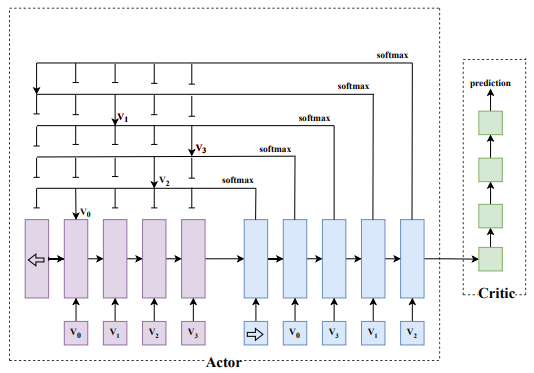
\includegraphics[scale=0.9]{pic/7.png}
        \caption{Actor-Critic网络结构}
    \end{figure}
\end{frame}

\begin{frame}{网络训练效果}
    \begin{figure}[htbp]
        \begin{minipage}{0.49\linewidth}
            \centering
            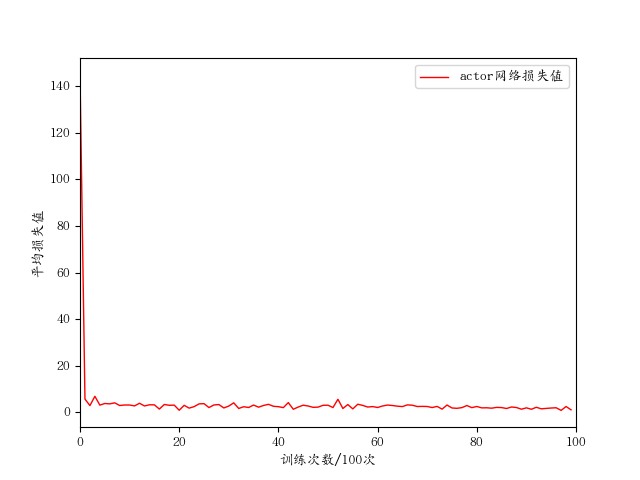
\includegraphics[scale=0.4]{pic/actor_x.png}
        \end{minipage}
        \begin{minipage}{0.49\linewidth}
            \centering
            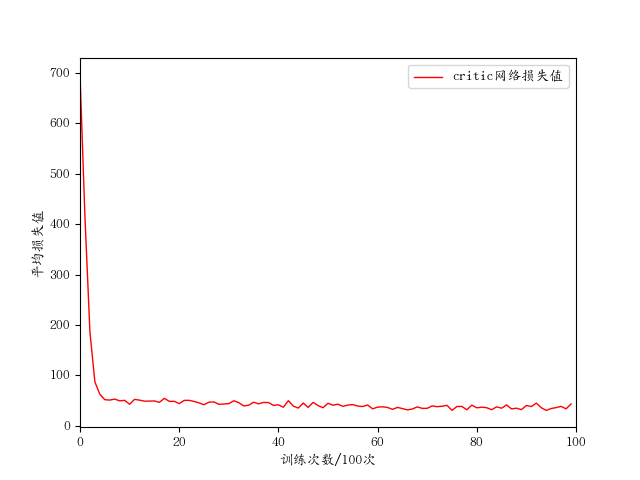
\includegraphics[scale=0.4]{pic/critic_x.png}
        \end{minipage}
        \caption{AC网络训练收敛效果}
    \end{figure}
\end{frame}

\begin{frame}{网络训练效果}

    \begin{figure}[htbp]
        \centering
        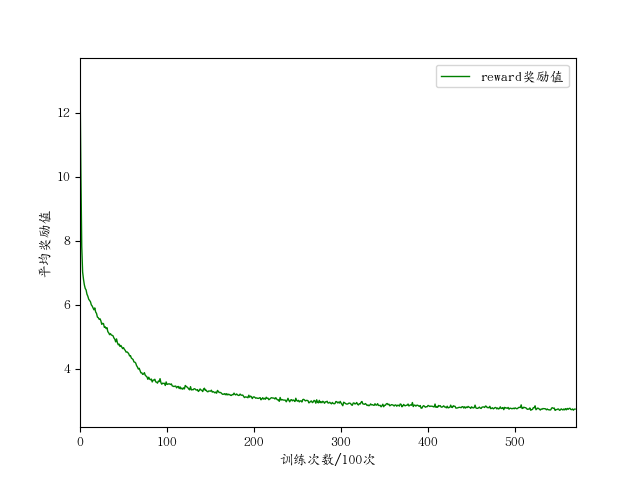
\includegraphics[scale=0.4]{pic/reward.png}
        \caption{AC算法负收益收敛效果}
    \end{figure}
\end{frame}

\begin{frame}{模型可视化展示}
    \begin{figure}[htbp]
        \centering
        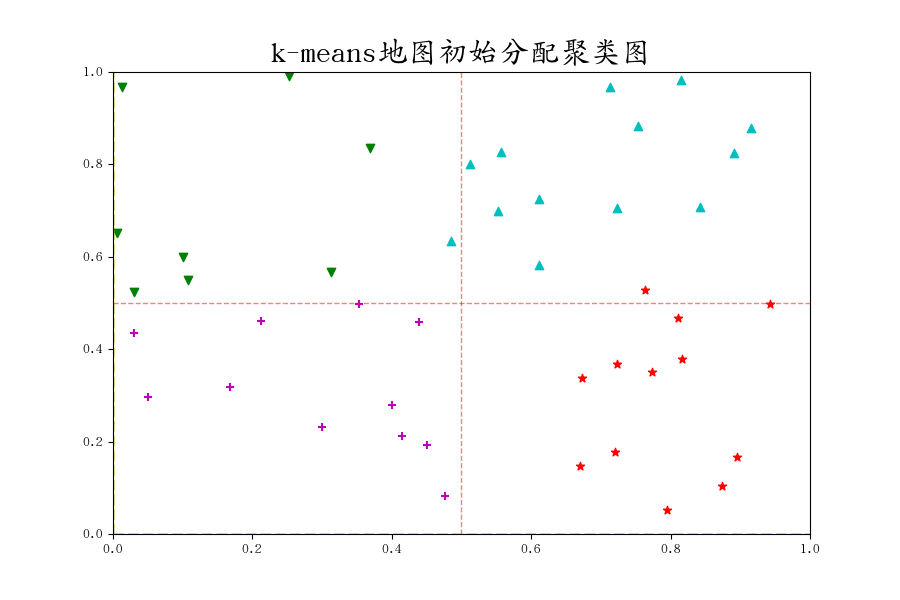
\includegraphics[scale=0.4]{pic/test1.png}
        \caption{k-means聚类初始分配地图}
    \end{figure}
\end{frame}

\begin{frame}{模型可视化展示}

    \begin{figure}[htbp]
        \centering
        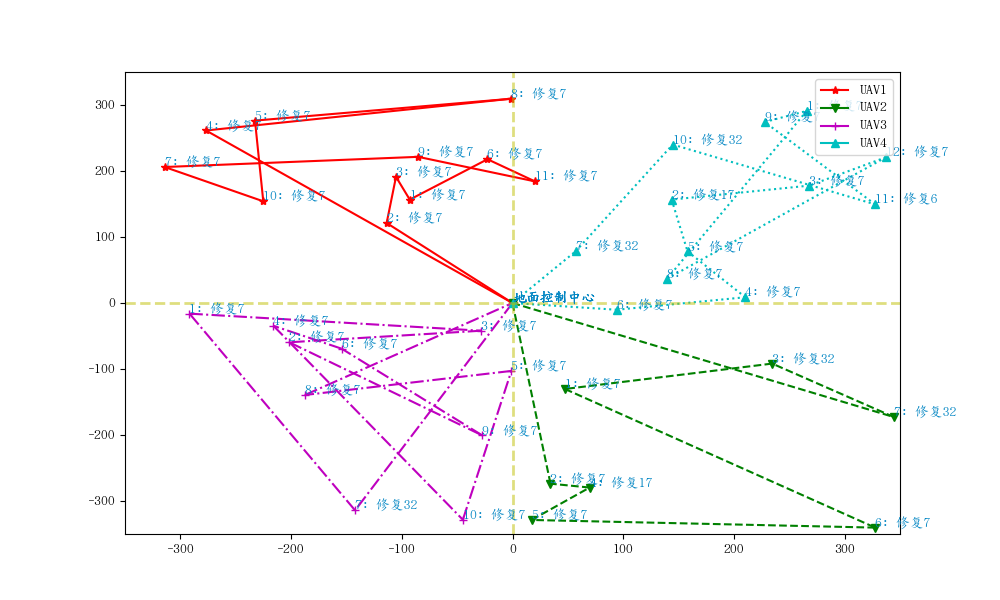
\includegraphics[scale=0.4]{pic/test2.png}
        \caption{无人机在700x700场地修复模拟}
    \end{figure}
\end{frame}

\section{参考文献}

\begin{frame}[allowframebreaks]
    \bibliography{ref}
    \bibliographystyle{njupt}
\end{frame}

\begin{frame}
    \begin{center}
        {\Huge\calligra Thanks!}
    \end{center}
\end{frame}

\end{document}